\begin{document}
	\chapter{Evaluation}
	This chapter discusses how the success criteria listed in the Preparation Chapter where achieved and exceeded.  Section \ref{Section: eval/ml} presents how the models' performance was evaluated on data extracted from a database of nodes and discusses the results of various metrics. In Section \ref{Section: eval/service-time} I analyse how the API as a whole would behave under real-life conditions and highlights the bottlenecks that I attempted to overcome through my implementation.
	\section{Success criteria} \label{Section: eval/success-criteria}
		This section describes how success criteria for the core project and extensions outlined in the project proposal (Appendix \ref{Appendix: Proposal}) have all been achieved and exceeded. Table \ref{Table: eval/success/status} highlights these achievements and their status. 
		\begin{longtable}{|p{.15\textwidth}|p{.3\textwidth}|p{.15\textwidth}|p{.3\textwidth}|}
			\hline
			& \textbf{Description} & \textbf{Status} & \textbf{Relevant section(s)} \\
			\hline
			\textit{Criterion 1} & Successfully implement a classification algorithm & \textbf{Successful} & Detailed in the Implementation Chapter - Section \ref{Section: impl/ml} \\
			\hline
			\textit{Criterion 2} & Evaluate the model and achieve $70\%$ in both precision and recall & \textbf{Successful} & Detailed results illustrated in the Evaluation Chapter - Section \ref{Section: eval/ml} \\
			\hhline{====}
			\multicolumn{4}{|c|}{\textbf{Extensions}} \\
			\hhline{====}
			\textit{Extension 1} & Implement and evaluate 3 other machine learning models, on top of the baseline classification algorithm & \textbf{Successful} & The implementation of these models is described in the Implementation Chapter - Section \ref{Section: impl/ml}. Their evaluation and results are detailed in the Evaluation Chapter - Section \ref{Section: eval/ml}.\\
			\hline
			\textit{Extension 2} & Comparatively evaluate the models and their relevance to the problem at hand & \textbf{Successful} & Detailed in the Evaluation Chapter - Section \ref{Section: eval/ml} \\
			\hline
			\textit{Extension 3} & Implement an automated feature extractor for the machine learning models & \textbf{Successful} & Detailed in the Implementation Chapter - Section \ref{Section: impl/neo4j} \\
			\hline
			\textit{Extension 4} & Embed the machine learning models into an API that can be used by the CADETS UI & \textbf{Successful} & Detailed in the Implementation Chapter - Sections \ref{Section: impl/overview} and \ref{Section: impl/REST}. \\
			\hline
			\caption{Status of success criteria and extensions.}
			\label{Table: eval/success/status}
		\end{longtable}
		
	\section{Evaluation of machine learning models} \label{Section: eval/ml}
		In this section, I will describe how the machine learning models were evaluated, show the results for the various metrics computed and discuss them, as well as their relevance to the problem I am trying to solve.
		
	\subsection{Evaluation methodology} \label{Section: eval/ml/methodology}
		In order to quantitatively evaluate the performance of the machine learning models implemented, I used a labelled dataset $\mathbf{s}$ containing $5,498$ nodes. Figure \ref{Fig: eval/ml/methodology/dist} shows how the labels and node types are distributed in the dataset used in this case. From there, we can observe that the node type distribution resembles the distribution that can be found in the general case in a provenance graph. Therefore, by evaluating the models on this dataset I can produce a comprehensive and accurate assessment of their performance. 
		\begin{figure}[H]
			\centering
			\begin{subfigure}{.4\textwidth}
				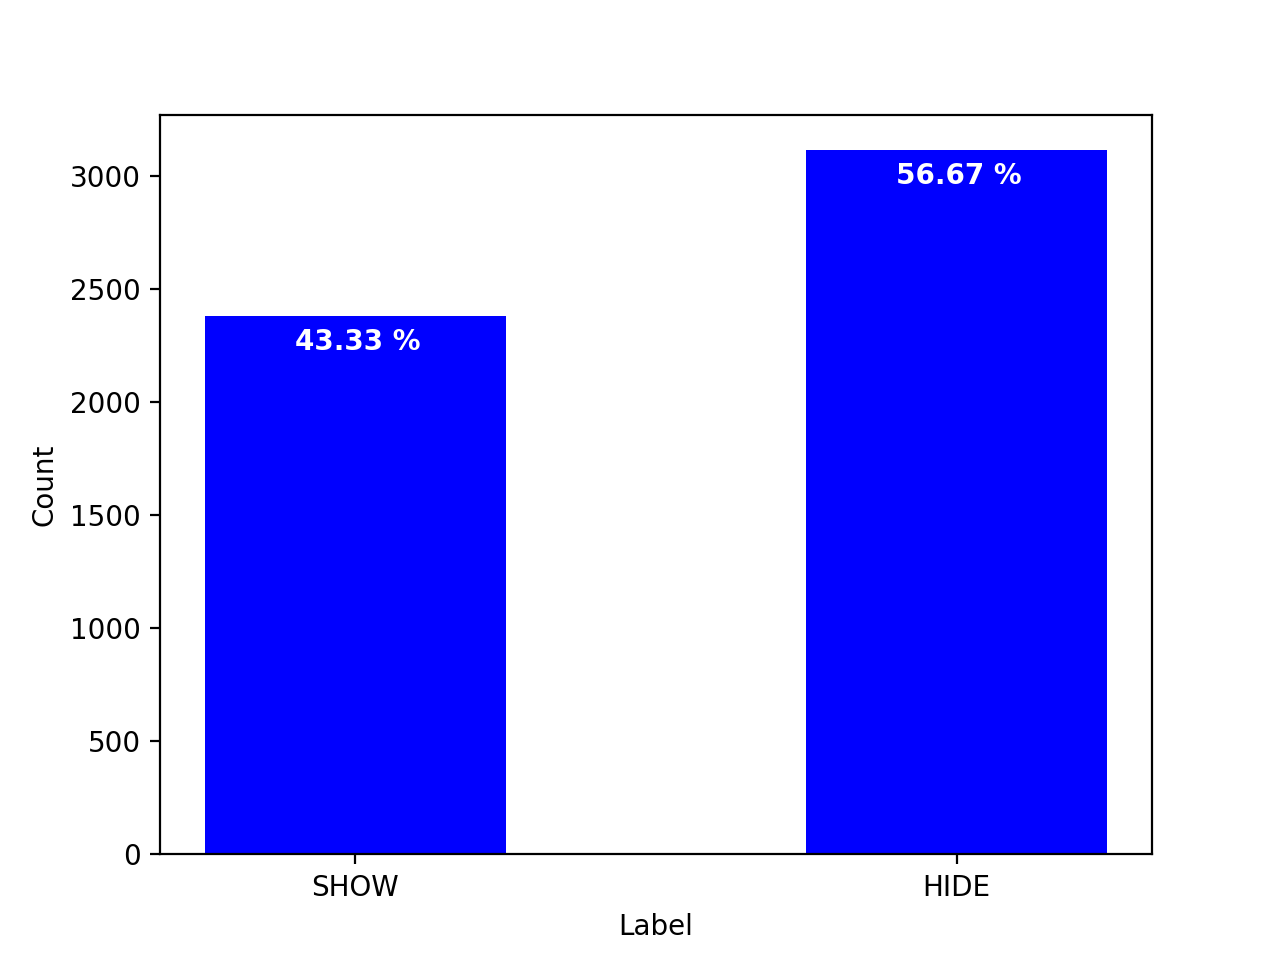
\includegraphics[width=\textwidth]{graphics/labels-dist}
			\end{subfigure}
			\hfill
			\begin{subfigure}{.4\textwidth}
				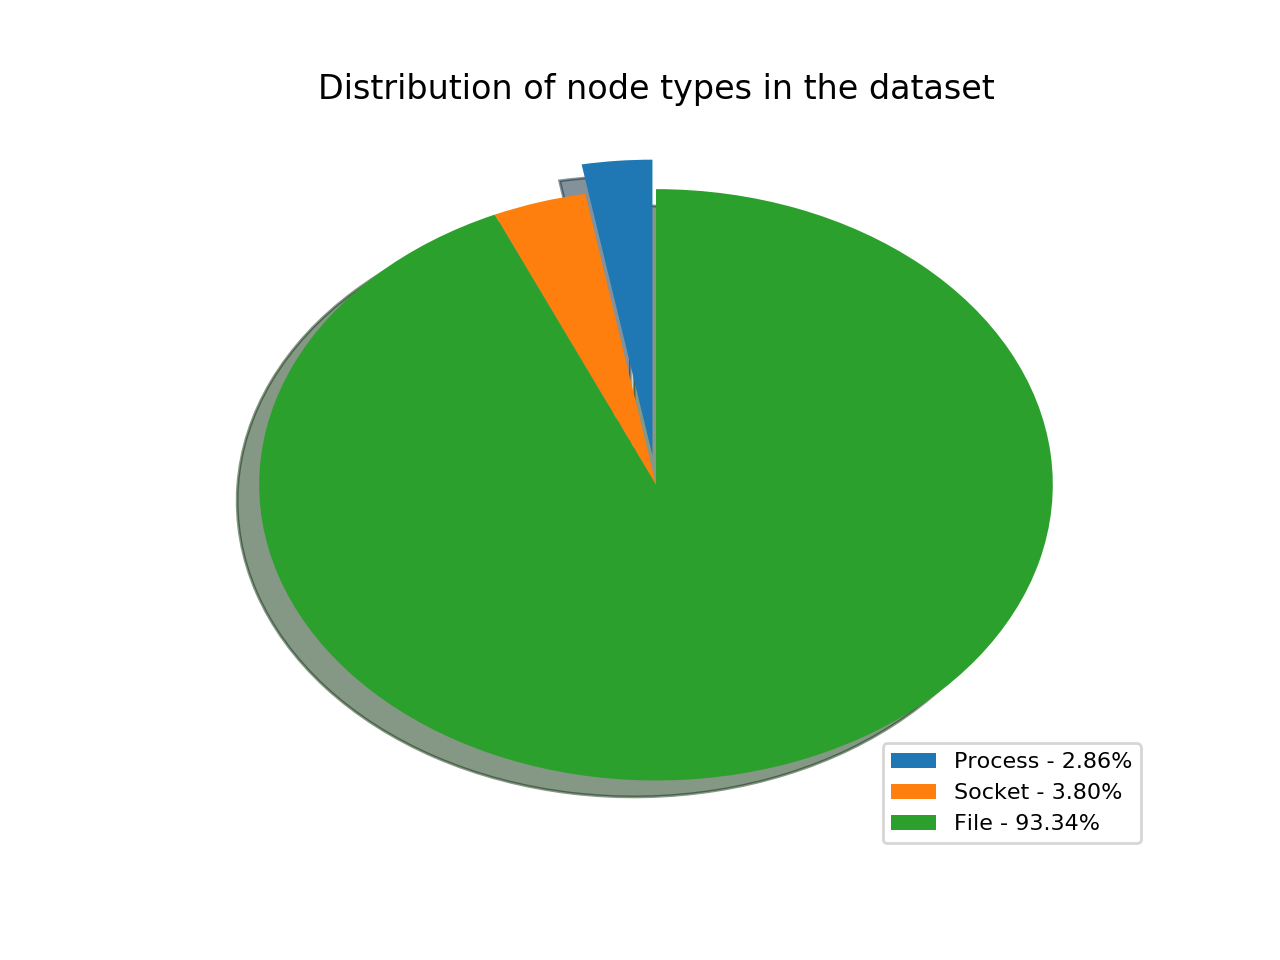
\includegraphics[width=\textwidth]{graphics/node-dist}
			\end{subfigure}
			\caption[Distributions of labels and node type in the dataset]{\textit{Left:} Distribution of the labels in the dataset. \textit{Right: }Distribution of the node types in the dataset.}
			\label{Fig: eval/ml/methodology/dist}
		\end{figure} 
		The technique used when evaluating the models was \textbf{10-fold outer Cross Validation}. Essentially, I split the dataset in $10$ equally-sized slots and use one at a time as a test set, while the other $9$ serve as the training set for the model. Figure \ref{Fig: impl/ml/methodology/kfold/first} shows how the dataset is divided in the first iteration of the cross-validation algorithm. This way, I ensure that none of the models is not tested on previously-seen examples and therefore I correctly evaluate how well they generalize on the given data.
		\begin{figure}[H]
			\centering
			\includegraphics[width=.8\textwidth]{graphics/k-fold}
			\caption{First step in k-fold cross validation}
			\label{Fig: impl/ml/methodology/kfold/first}
		\end{figure}
		
		At every iteration, I compute a set of metrics that for estimating the model's performance and the final result for every metric in part is given by averaging over the values obtained. 
	\subsection{Metrics involved} \label{Section: eval/ml/metrics}
	
		In this section, I will outline the metrics used when evaluating the machine learning models. The choice of good metrics is essential when comparatively evaluating a number of machine learning models. The simplest metric for evaluating of classification algorithms is \textbf{accuracy}, and can be computed using the formula: 
		\\
		\begin{equation}
			acc = \frac{\text{no. of correctly predicted nodes}}{\text{total no. of predicted nodes}}
		\end{equation}
		\\
		Accuracy, however, is not efficient when it comes to imbalanced data, as it is the case here(i.e. we have a $43\%/57\%$ \textit{SHOW/HIDE} distribution amongst the nodes). Therefore, more complex metrics are required in order to correctly assess the performance of the models implemented. These metrics are based on the notions of \textit{true positives, true negatives, false positives and false negatives}, which can easily be illustrated using a confusion matrix, such as the one from Figure \ref{Fig: eval/ml/metrics/confusion-matrix}.
		\begin{figure}[H]
			\centering
			\includegraphics[width=.7\textwidth]{graphics/confusion-matrix}
			\caption{Confusion matrix for two-class classification}
			\label{Fig: eval/ml/metrics/confusion-matrix}
		\end{figure}
		The metrics I used to evaluate the general performance of the models are presented in Table \ref{Table: eval/ml/metrics/metrics}. From those, the F1 score and the MCC are the most meaningful for this case, as they ignore the fact that the data is not balanced. The MCC gives a value between $[-1, 1]$, where $1$ represents perfect prediction, $0$ not better than random and $-1$ a total disagreement between the predicted and true labels.
		\begin{longtable}{|p{.15\textwidth}|p{.40\textwidth}|c|}
		   \textbf{Metric} & \textbf{Intuition} &\textbf{Formula} \\
			\hline
			\textit{Precision} & fraction of nodes correctly labelled as \textit{SHOW} in all nodes classified. & {$\centering \text{precision} = \frac{tp}{tp+fp}$} \\
			\hline 
			\textit{Recall} & fraction of \textit{SHOW} nodes correctly classified. & $\text{recall} = \frac{tp}{tp+fn}$ \\
			\hline
			\textit{F3 score} & takes into consideration both the precision and the recall of the model in order to assess its performance & $\text{F3} = 10\times\frac{\text{precision}\times\text{recall}}{9\times\text{precision} + \text{recall}}$\\
			\hline 
			\textit{Matthew's Correlation Coefficient (MCC)} & takes into account true and false positives and negatives in order to provide a balanced metric for the model's performance & $MCC = \frac{tp\times tn - fp\times fn}{\sqrt{(tp+fp)\times(tp+fn)\times(tn+fp)\times(tn+fn)}}$\\
			\hline
			\caption{Machine learning evaluation metrics}
			\label{Table: eval/ml/metrics/metrics}
		\end{longtable}
		
		I chose to use the F3 score instead of the more frequently encountered F1, because it weights the recall of the models more favourably than their precision. I am interested in having a high recall of the model because, in practice, I want the models to show as many of the nodes that are of interest as possible, even if this results in a lower precision. The F3 score gives a value in $[0, 1]$, with $F3 = 0$ representing a total disagreement between the classification results and the true labels and $F3 = 1$ representing a perfect classification.
		
		\subsection{Results \& discussion} \label{Section: eval/ml/results}
		In this section I will present and discuss the results obtained as part of the evaluation. Table \ref{Table: eval/models/results/overall} shows the averaged scores obtained by the four models implemented as part of the project. 
		
		\begin{longtable}{|p{.15\textwidth}|p{.18\textwidth}|p{.18\textwidth}|p{.18\textwidth}|p{.18\textwidth}|}
			\hline
			& \textbf{Logistic Regression} & \textbf{MLP} & \textbf{PNN} &  \textbf{CNN}\\
			\hline
			\textit{Accuracy} & $91.48 \pm 0.90 \%$ &$91.87 \pm 1.35 \%$  &  $91.94 \pm 1.26 \%$ &\cellcolor{green!50}  $\mathbf{93.74 \pm 6.5 \%}$ \\
			\hline
			\textit{Precision} & $97.81 \pm 0.81\%$& $98.23 \pm 3.41 \%$ &   $89.27 \pm 2.13 \%$ & \cellcolor{green!50} $\mathbf{97.28 \pm 1.10 \%}$  \\
			\hline
			\textit{Recall} & $86.92 \pm 1.60\%$& $86.85 \pm 3.98 \%$ & $92.51 \pm 1.15 \%$ & \cellcolor{green!50} $\mathbf{91.52 \pm 1.51 \%}$  \\
			\hline
			\textit{F3 score} & $87.90 \pm 1.46 \%$ & $87.83 \pm 3.37 \%$  &  $92.17 \pm 1.17 \%$ & \cellcolor{green!50} $\mathbf{92.06 \pm 1.31 \%}$\\
			\hline
			\textit{MCC} & $83.62 \pm 1.65\%$& $84.13 \pm 2.29 \%$ &  $83.70 \pm 2.53 \%$ & \cellcolor{green!50} $\mathbf{87.59 \pm 1.30 \%}$\\
			\hline
			\caption{Evaluation results for the models implemented.}
			\label{Table: eval/models/results/overall}
		\end{longtable}
		By analysing the results above, I can conclude that the Convolutional Neural Network is significantly more performant than the others, with an MCC score of $\mathbf{87.59 \pm 1.30 \%}$. Moreover, it high values for both recall (and therefore it is very likely to return all the relevant nodes)  and precision (making it an effective filtering algorithm). The PNN has an even higher recall value, classifying more of the relevant results as \textit{SHOW}. Its low precision, however, makes it a poor filtering tool, as the analyst would have to search through a larger node space.
		\\ \\
		The bar graph in Figure \ref{Fig: eval/ml/results/MCC-per-fold} illustrates a fold-by-fold breakdown of the MCC results for all 4 models. It supports the previous conclusion (i.e. that the CNN is the most performant model), as it has a higher MCC model than the other models for $8/10$ folds and therefore it generalizes better than them.    
		\begin{figure}[H]
			\centering
			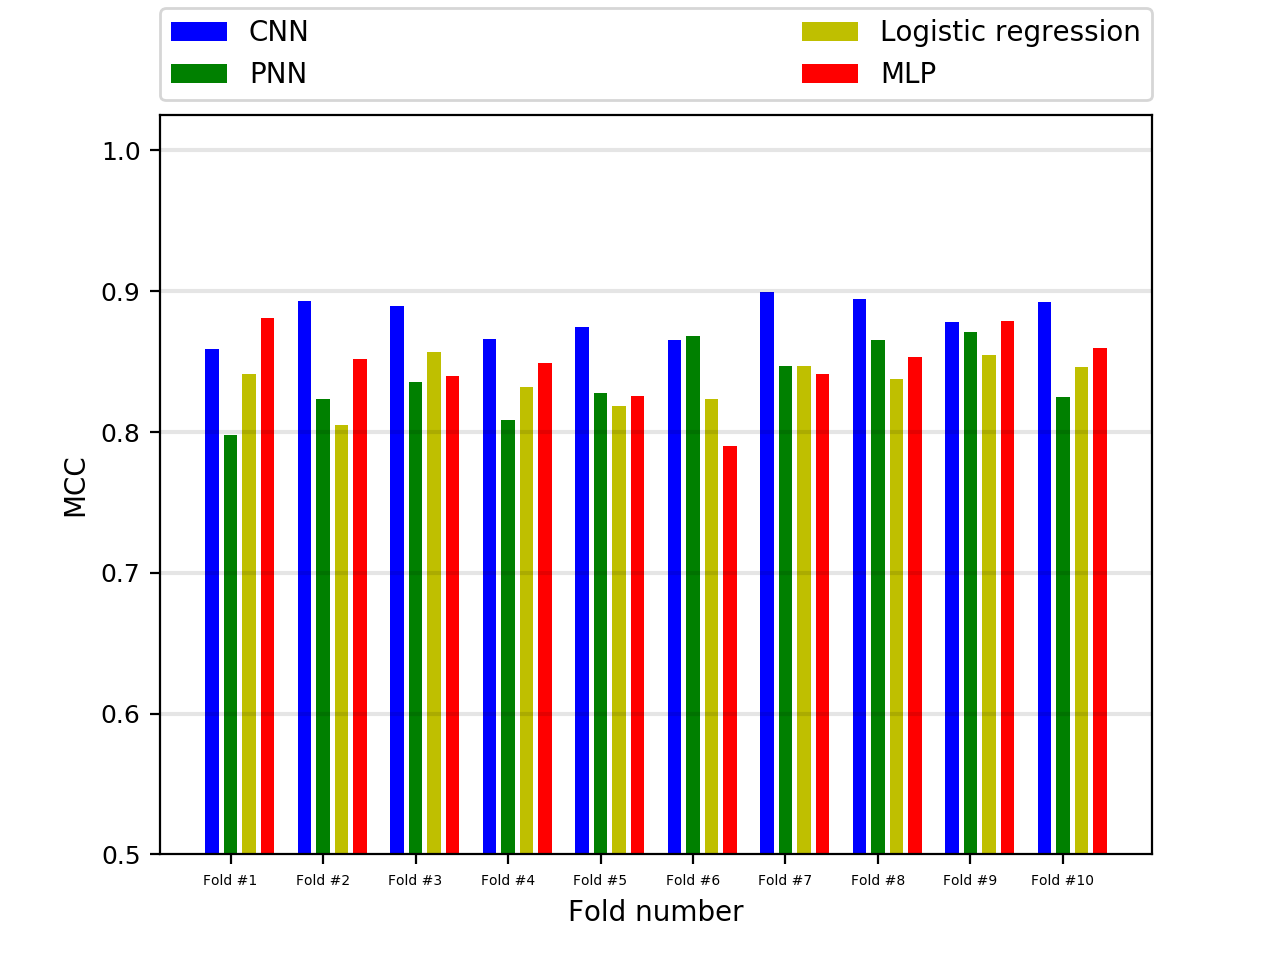
\includegraphics[width=\textwidth]{graphics/MCC-per-fold}
			\caption{Comparative MCC at every fold.}
			\label{Fig: eval/ml/results/MCC-per-fold}
		\end{figure}
		Figure \ref{Fig: eval/ml/results/ROC} illustrates the averaged ROC curves of every model, obtained by interpolating over the 10 folds of the Cross Validation algorithm. The ROC curve of the CNN is the steepest, indicating the fact that it has the highest ability of discriminating between the two classes (i.e. \textit{SHOW} and \textit{HIDE}). Furthermore, this fact is shown by its ROC-AUC score\footnote{Represented by the area under the ROC curve.}, which is larger than the one for the other models.
		\\ \\
		Concavities present in all the curves indicate the fact that, locally, the models have worse than random behaviour. Therefore, even if all the models have a good general performance, they cannot fit the data perfectly. This is a possible consequence of the fact that the models are trying to fit a set of $6$ ground-truths at a time and that each of these rules has a different number of nodes representing them. In other words, this is caused by the fact that the models fit some rules better than others. 
		\begin{figure}[H]
			\centering
			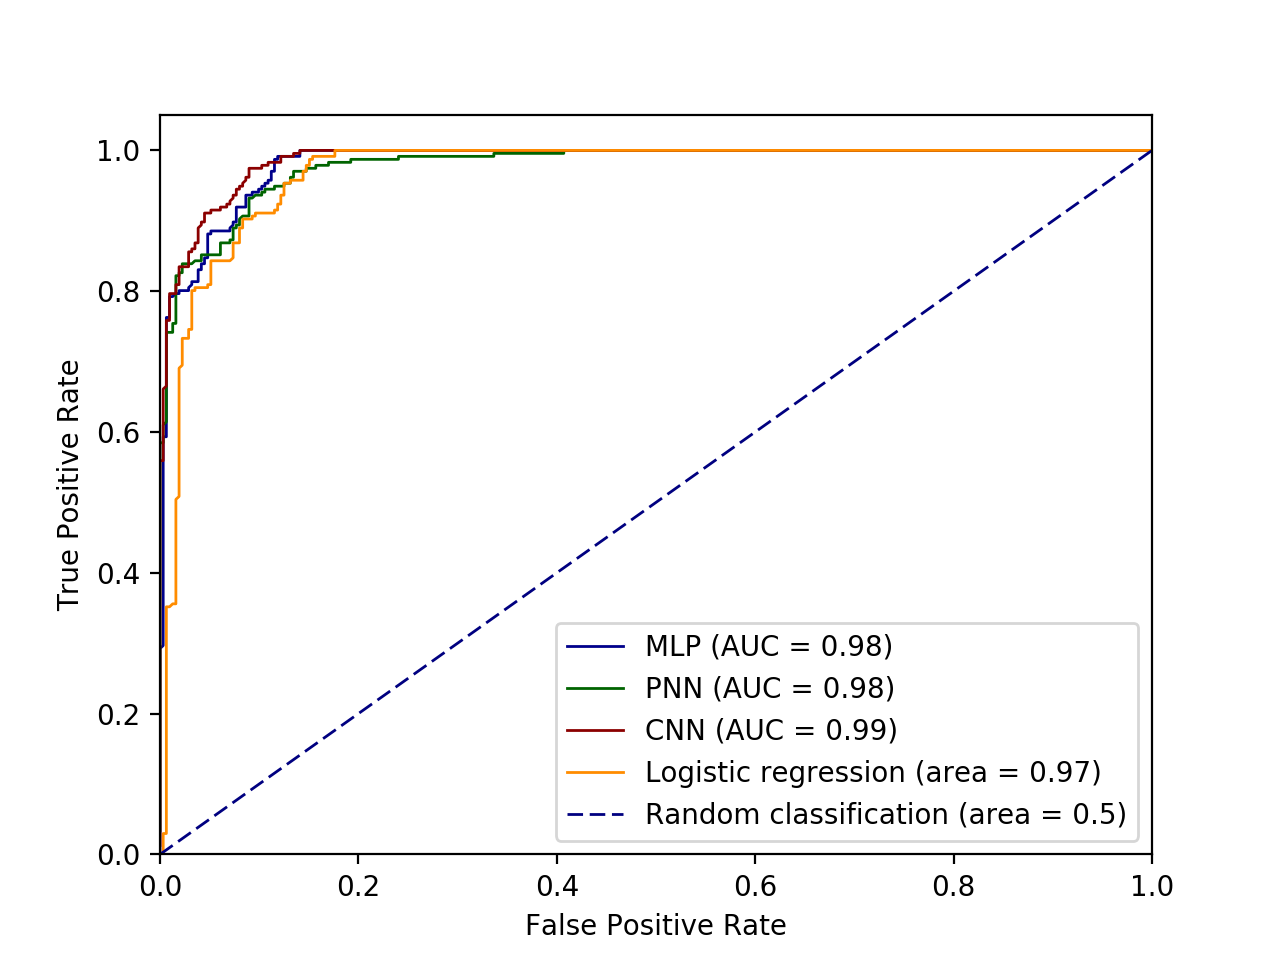
\includegraphics[width=\textwidth]{graphics/ROC-curve}
			\caption{Mean ROC curves obtained after 10-fold outer-CV}
			\label{Fig: eval/ml/results/ROC}
		\end{figure}
		The precision-recall curves for the models implemented from Figure \ref{Fig: eval/ml/results/precision-recall} shows the tradeoff between precision and recall for different probability thresholds. The \textbf{average precision} (AP) summarizes each of the plots as the weighted mean of precisions at each threshold, with the recall difference compared to the previous threshold as the weight:
		\begin{equation}
			AP = \sum_{n} (R_n - R_{n-1}) P_n
		\end{equation}
		where $R_n$ and $P_n$ are the precision and recall at the $n^{th}$ threshold. 
		\\ \\
		From their analysis, we can observe that the CNN(Figure \ref{Fig: eval/ml/results/precision-recall/cnn}) has the highest average precision (AP = $0.98$) and therefore can be a highly effective filtering tool. The PNN (Figure \ref{Fig: eval/ml/results/precision-recall/pnn}) has a precision close to $1$ for recall values of up to $\approx 0.8$, but then drops steeply, causing a lower value for the average precision (AP = $0.96$). 
		\\ \\
		The other two models also have lower AP (i.e. $0.95$ for logistic regression and $0.96$ for the MLP), indicating a lower performance. Moreover, the precision-recall curve for the logistic regression algorithm is highly inconsistent and therefore is the least performant of the four models. This fits my expectations, as it is the most simplistic model and cannot identify complex relationships between the features I use to represent the nodes.
		\begin{figure}[H]
			\centering
			\begin{subfigure}{.4\textwidth}
				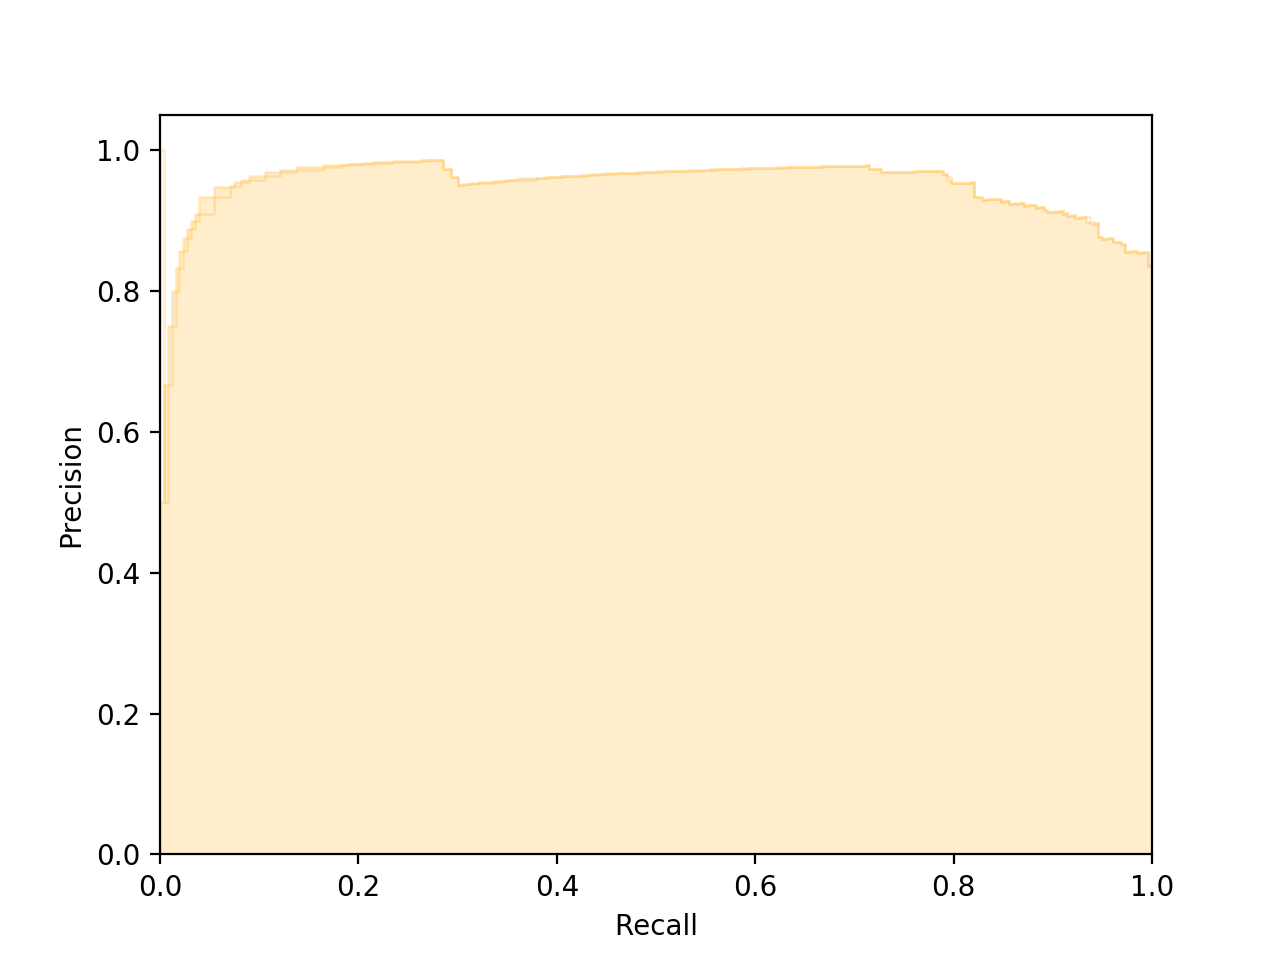
\includegraphics[width=\textwidth]{graphics/precision-recall/logreg}
				\caption{Precision-recall curve for logistic regression. AP = $0.95$}
				\label{Fig: eval/ml/results/precision-recall/logreg}
			\end{subfigure} \hfill
			\begin{subfigure}{.4\textwidth}
				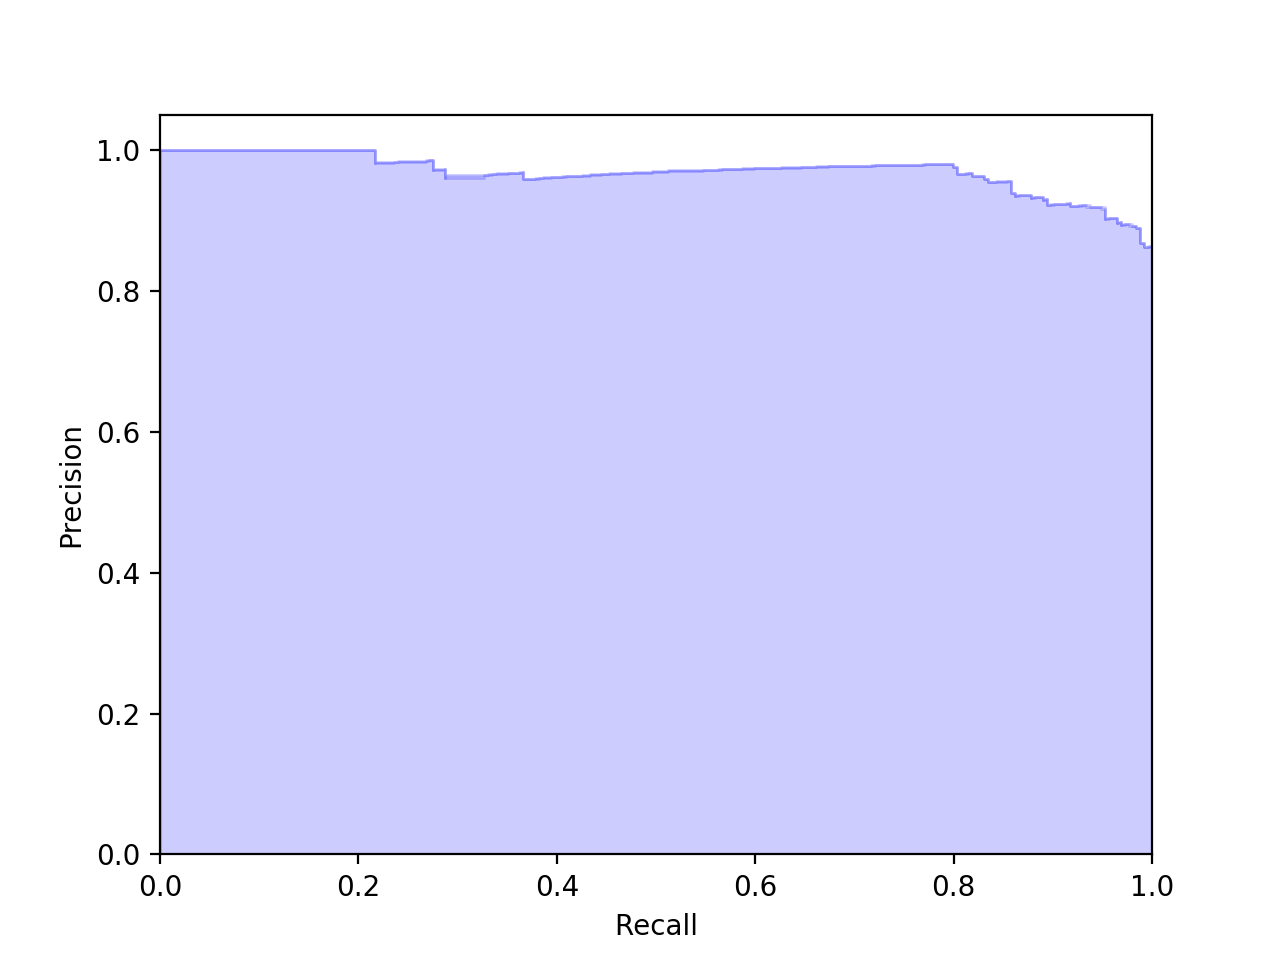
\includegraphics[width=\textwidth]{graphics/precision-recall/mlp}
				\caption{Precision-recall curve for MLP.  AP = $0.96$}
				\label{Fig: eval/ml/results/precision-recall/mlp}
			\end{subfigure}
			\begin{subfigure}{.4\textwidth}
				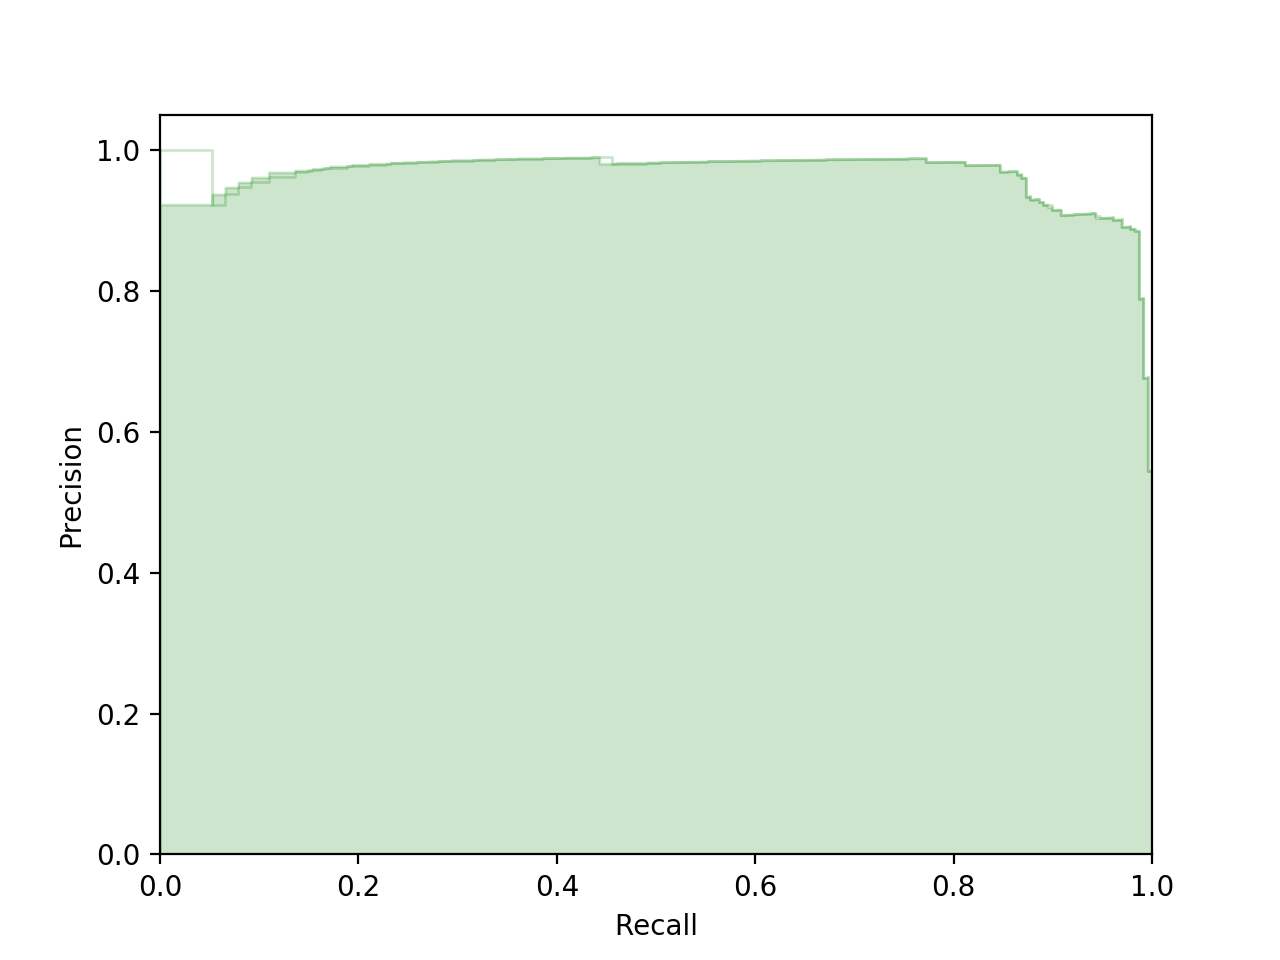
\includegraphics[width=\textwidth]{graphics/precision-recall/pnn}
				\caption{Precision-recall curve for PNN. AP = $0.96$}
				\label{Fig: eval/ml/results/precision-recall/pnn}
			\end{subfigure} \hfill
			\begin{subfigure}{.4\textwidth}
				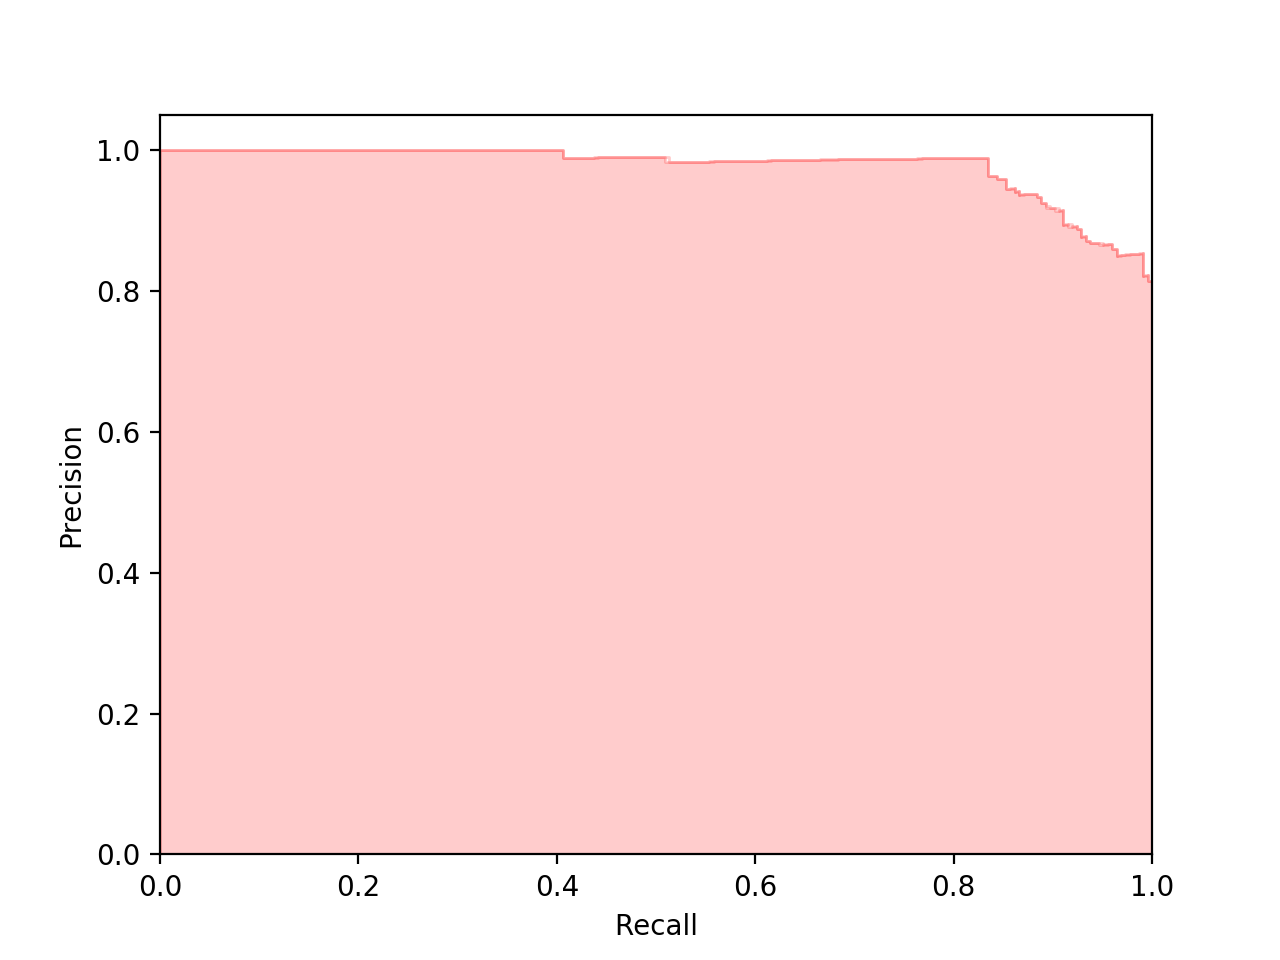
\includegraphics[width=\textwidth]{graphics/precision-recall/cnn}
				\caption{Precision-recall curve for CNN. AP = $0.98$}
				\label{Fig: eval/ml/results/precision-recall/cnn}
			\end{subfigure}
			\caption{Average precision-recall curves for the 4 models.}
			\label{Fig: eval/ml/results/precision-recall}
		\end{figure}
			In conclusion, all four models have a reasonable performance on the data used during evaluation, meeting the success criterion outlined in the Project Proposal (i.e. achieving over $70\%$ in both precision and recall). As expected, the Convolutional Neural Network is the most performant of the models, with an MCC = $87.59 \pm 1.30 \%$ and F3 = $92.06 \pm 1.31 \%$, despite the highly imbalanced data.
			
		\section{Service time evaluation} \label{Section: eval/service-time}
			This project is meant to be a complete API that can be used in practice by the CADETS user interface. Therefore, besides the performance of the machine learning model used, it is essential to evaluate it in terms of the service speed as well. All the timing results were obtained using my personal machine. For a job processing $N$ nodes, the service time is calculated using the following formula:  
			\begin{equation}
				\text{service\_time} = N\times [CCT + CHR \times CET + (1-CHR) \times (CT + RCT)] + MLT
				\label{Eq: eval/service-time/overall}
			\end{equation}
			where: 
			\begin{itemize}
				\item $\mathbf{CCT} \in \mathbb{R}$ = Cache Check Time - time taking to check if a node is in the cache database and if the entry is still valid.
				\item $\mathbf{CHR} \in [0, 1]$ = Cache Hit Rate.
				\item $\textbf{CET} \in \mathbb{R}$ = Cache Extraction Time - time taking to extracted one cached result.
				\item $\textbf{CT} \in \mathbb{R}$ = Classification Time - time taking to classify a node. 
				\item $\textbf{RCT} \in \mathbb{R}$ = Result Caching Time - time required to add a new classification result to the cache database.
				\item $\mathbf{MLT} \in \mathbb{R}$ = Model Loading Time - time required to configure the model (i.e. defining its components and load the corresponding pre-optimised parameters)
			\end{itemize}
			In practice, the API is expected to re-use many of the classification results. For this reason, I assume the the cache to have a hit-rate $CHR = 90\%$. For simulation purposes, the database was populated with $10, 000$ nodes and $30$ completed jobs, each having processed $1, 000$ nodes. 
			\\ \\
			The first step performed by the application when the new job is initiated is to check the cache and try to get the nodes that are cached. In this given simulation environment, the Cache Check Time, Cache Extraction Time and Result Caching Time are $CCT=0.01s$, $CET=0.02s$ and $RCT=0.01s$, respectively.  
			
		\subsection{Classification timings} \label{Section: eval/service-time/classification}
			The classification time is not as straight-forward as the times shown so far. It was computed using the following formula:
			\begin{equation}
				CT = NTT + FET + MRT
			\end{equation}
			where: 
			\begin{itemize}
				\item $\mathbf{NTT} \in \mathbb{R}$ = Node Type Time - time required to get the node type
				\item $\mathbf{FET} \in \mathbb{R}$ = Feature Extraction Time - time required to extract the features required for a node.
				\item $\mathbf{MRT} \in \mathbb{R}$ = Model Running Time - time required for the model to produce a classification result for a node.
			\end{itemize}
			If a node is not in the cache, we first need to get the node type. The feature extraction time is dependent on this, as different node types require a slightly different feature extraction algorithm. Moreover, for a \textit{Meta} or \textit{Pipe} node, we also need to look for the closest \textit{Process} node to them. Table \ref{Table: eval/service-time/classification/fet} shows a breakdown of these timings\footnote{The time values were estimated by averaging over 100 runs of the feature extractor, with 20 nodes each.}, when the nodes are extracted from a database of $6,008$ nodes and taking into account the policy defined in Section \ref{Section: impl/REST/actual} from the Implementation chapter.
			\begin{longtable}{|p{.1\textwidth} || p{.15\textwidth} | p{.20\textwidth}| p{.15\textwidth}| p{.20\textwidth} | }
				\textbf{Node type} & \textbf{NTT} (s) & \textbf{Time for finding the closest node} (s)& \textbf{FET} (s)& \textbf{Total FET} (s)\\
				\hline
				\textit{File} & \multirow{5}{*}{$0.13$}& $0.0$ & $0.78$& $\mathbf{0.91}$ \\
				\hhline{-~---}
				\textit{Process} & & $0.0$ & $0.83$ & $\mathbf{0.96}$\\
				\hhline{-~---}
				\textit{Socket} & & $0.0$ & $0.67$ & $\mathbf{0.80}$ \\
				\hhline{-~---}
				\textit{Pipe} & & $0.01$ & $0.83$ & $\mathbf{0.97}$ \\
				\hhline{-~---}
				\textit{Machine} & & $0.0$ & $0.0$ & $\mathbf{0.13}$\\
				\hline
				\caption{Breakdown of feature extraction times}
				\label{Table: eval/service-time/classification/fet}
			\end{longtable}		
			Once the feature vectors are computed, they are passed to the machine learning models to be classified. Based on the model type, this task can take different amounts of time. The classification time can then be written as a function of node and model type as follows: 
			\begin{equation}
				CT(nt, mt) = Total\_FET(nt) + MRT(mt)
			\end{equation}
			By using the node type distribution outlined in the histogram from Figure \ref{Figure 2.1.1}, one can compute the average feature extraction time as follows:
			\begin{equation}
				\hat{FET} = \sum_{nt\in \mathbf{\mathcal{N}}} (\mathbb{P}(nt) \times Total\_FET(nt))
			\end{equation} 
			where $\mathcal{N}$ is the set of available node types. When plugging in the numbers, we get $\hat{FET} = 0.89\text{s}$. Using this, the average classification time as a function of model type can be written as: 
			\begin{equation}
				\hat{CT}(mt) =  \hat{FET} + MRT(mt) 
			\end{equation}  
			 Table \ref{Table: eval/service-time/classification/CT} shows the resulting $MLT$, $MRT$  and $\hat{CT}$ for each model.
			
			\begin{longtable}{|p{.15\textwidth}||p{.15\textwidth}|p{.15\textwidth}|p{.15\textwidth}|p{.15\textwidth}|}
				\textbf{Model} & \textit{Logistic Regression} & \textit{MLP} & \textit{CNN} & \textit{PNN} \\
				\hline
				$\mathbf{MLT}$ (s) & $0.01$ & $0.02$ & $0.02$ & $0.01$  \\
				\hline
				$\mathbf{MRT}$ (s) & $0.01$ &$0.01$ & $0.01$ & $0.09$ \\
				\hline\hline
				$\mathbf{\hat{CT}}$ (s) & $\mathbf{0.90}$ & $\mathbf{0.90}$ & $\mathbf{0.90}$ & $\mathbf{0.99}$ \\
				\hline
				\caption{Breakdown of average classification times.}
				\label{Table: eval/service-time/classification/CT}
			\end{longtable} 
			
			\subsection{Bringing it all together} \label{Section: eval/service-time/together}
			Now that I have computed all the individual time values, I can bring them all together and compute the \textit{service time}, using Eq. \ref{Eq: eval/service-time/overall}. Table \ref{Table: eval/service-time/together/overall} shows the resulting service times for different model types, taking the number of nodes $N=1,000$.
			\begin{longtable}{|p{.13\textwidth}||p{.08\textwidth}|p{.08\textwidth}|p{.08\textwidth}|p{.08\textwidth}|p{.08\textwidth}|p{.08\textwidth}|p{.08\textwidth}||p{.1\textwidth}|}
				\textbf{Model} & \textbf{N} & \textbf{CHR}  &\textbf{CCT} (s) & \textbf{CET} (s) & \textbf{RCT} (s)& $\mathbf{\hat{CT}}$ (s)& \textbf{MLT} (s) & \textbf{Total} (s)\\
				\hline
				\textit{Logistic Regression} & \multirow{5}{*}{$1000$} & \multirow{5}{*}{$0.90$} & \multirow{5}{*}{$0.01$} & \multirow{5}{*}{$0.02$} & \multirow{5}{*}{$0.01$} & $0.90$ & $0.01$ & \cellcolor{green!20} $\mathbf{119.01}$ \\
				\hhline{-~~~~---}
				\textit{MLP} &  &  &   & &  & $0.90$ & $0.02$ &\cellcolor{green!20} $\mathbf{119.02}$  \\
				\hhline{-~~~~---}
				\textit{CNN} &  &  &  & &  & $0.90$ & $0.02$ & \cellcolor{green!20} $\mathbf{119.02}$ \\
				\hhline{-~~~~---}
				\hhline{-~~~~---}
				\textit{PNN} &  &  &  & &  & $0.99$ & $0.01$ & \cellcolor{green!20} $\mathbf{128.01}$ \\
				\hline
				\caption{Service time analysis results}
				\label{Table: eval/service-time/together/overall}
			\end{longtable}
			
			From the table above we can observe that there is little difference between the models when it comes to the overall running time of the API. When using the PNN as the classifier, the API takes the most time to run. This is a consequence of the fact that the number of vector operations that need to be performed by it is directly proportional to the number of training samples provided, unlike the other models, which all have a finite number of neurons. 
			\\ \\
			Another key observation is the fact that, in all cases, the classification time $\hat{CT}$ is considerably higher than all the other timings. To be more precise, the feature extraction step is the most impactful in this case. This is given by the poor performance of the $3^{rd}$ party library that supports the connection to the Neo4J database and represents a significant bottleneck for the performance of the model implemented. In order to overcome this issue, I decided to use a cache database for the API, by relying on the fact that the classification  results are unlikely to change over time. In order to better illustrate the impact of the caching mechanism, I will first define the service time formula for a non-caching API as follows:
			\begin{equation}
				service\_time = N \times \hat{CT} + MLT
			\end{equation}
			Based on this formula, I created the bar chart from Figure \ref{Fig: eval/service-time/bringing/bar}, which illustrates the difference in service time between an API using a cache database with $CHR=0.90$ and an API that is not using a cache (i.e. it simply classifies every node for a given job). From it we can clearly observe that, when using a cache, the API is several orders of magnitude more time efficient than when simply classifying node in a request. Therefore, the cache database can be considered as an efficient solution for overcoming the bottleneck posed by the feature extraction step.  
			\begin{figure}[H]
				\centering
				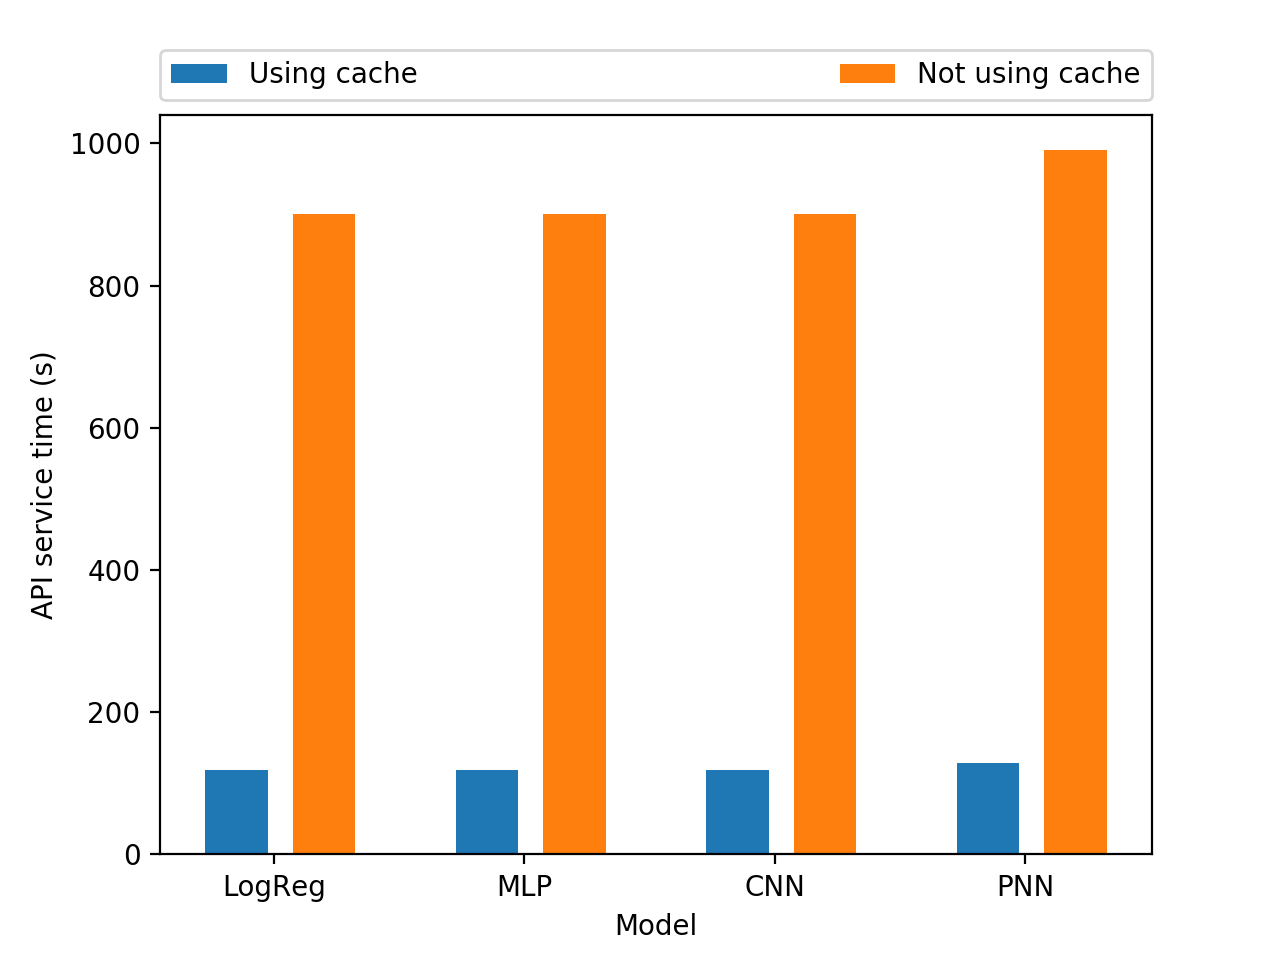
\includegraphics[width=.7\textwidth]{graphics/service-time-hist}
				\caption{Bar chart of the service times with/ without using cache for $1,000$ nodes. For the cached version, I considered $CHR=0.90$}
				\label{Fig: eval/service-time/bringing/bar}
			\end{figure}
			However, even though the cache database partially solves the feature extractor limitation, the service time of the API is still high. For this reason, I decided to implement the 2-step format of the REST API described in Section \ref{Section: impl/REST/actual}.
		\section{Summary} \label{Section: eval/summary}
			Initially, this chapter listed the success criteria for this project and how they were achieved. Following this, I described how the models implemented met the expected performance and, through comparative evaluation, shown the fact that the CNN outperforms the logistic regression, MLP and PNN on the dataset built from the graph database. In the end, I evaluated the tool from a service-time point of view and shown the bottlenecks that were encountered and motivated some of my implementation decisions. 
\end{document}